\section{Spec 11 --- Bias audit}

\begin{table}[htbp]
\centering\small
\caption{Bias audit summary (Gini: 0 = equal, 1 = one unit has everything).}
\label{tab:bias}
\begin{tabular}{lp{0.68\columnwidth}}
\toprule
Dimension & Finding \\
\midrule
Geography & 148 countries; Sweden, US and Switzerland hold 37\% of records (Gini 0.91); Africa, South Asia and South
America nearly absent; Latvia only 264 records. \\
Language & Swedish, English and Finnish are 72\% of the notes (Gini 0.82). \\
Season & Summer 37\%, spring 29\%, autumn 20\%, winter 15\%. \\
Users & The top 1\% of users wrote 20--61\% of a platform's records (Gini 0.65--0.88); CrowdWater has no user id. \\
\bottomrule
\end{tabular}
\end{table}

The corpus is significantly biased (Table~\ref{tab:bias}, Figures~\ref{fig:map} and~\ref{fig:months}). 
This is partly a result of our own collection choices, since iNaturalist was collected for 14 countries and three sources are national portals.
Only CrowdWater and EyeOnWater are global. Records peak mostly in summer, meaning that winter states such as ice are rare (only two gold records).
Additionally, on Laji.fi, about nine people (the top 1\% of users) wrote 61\% of the records, so in the Finnish text, the abbreviations they
use dominate. This means that the results on CSWO-Bench should be reported per platform and language, and shouldn't be transferred to other regions, 
seasons or languages without previous analysis.



\begin{figure}[htbp]
\centering
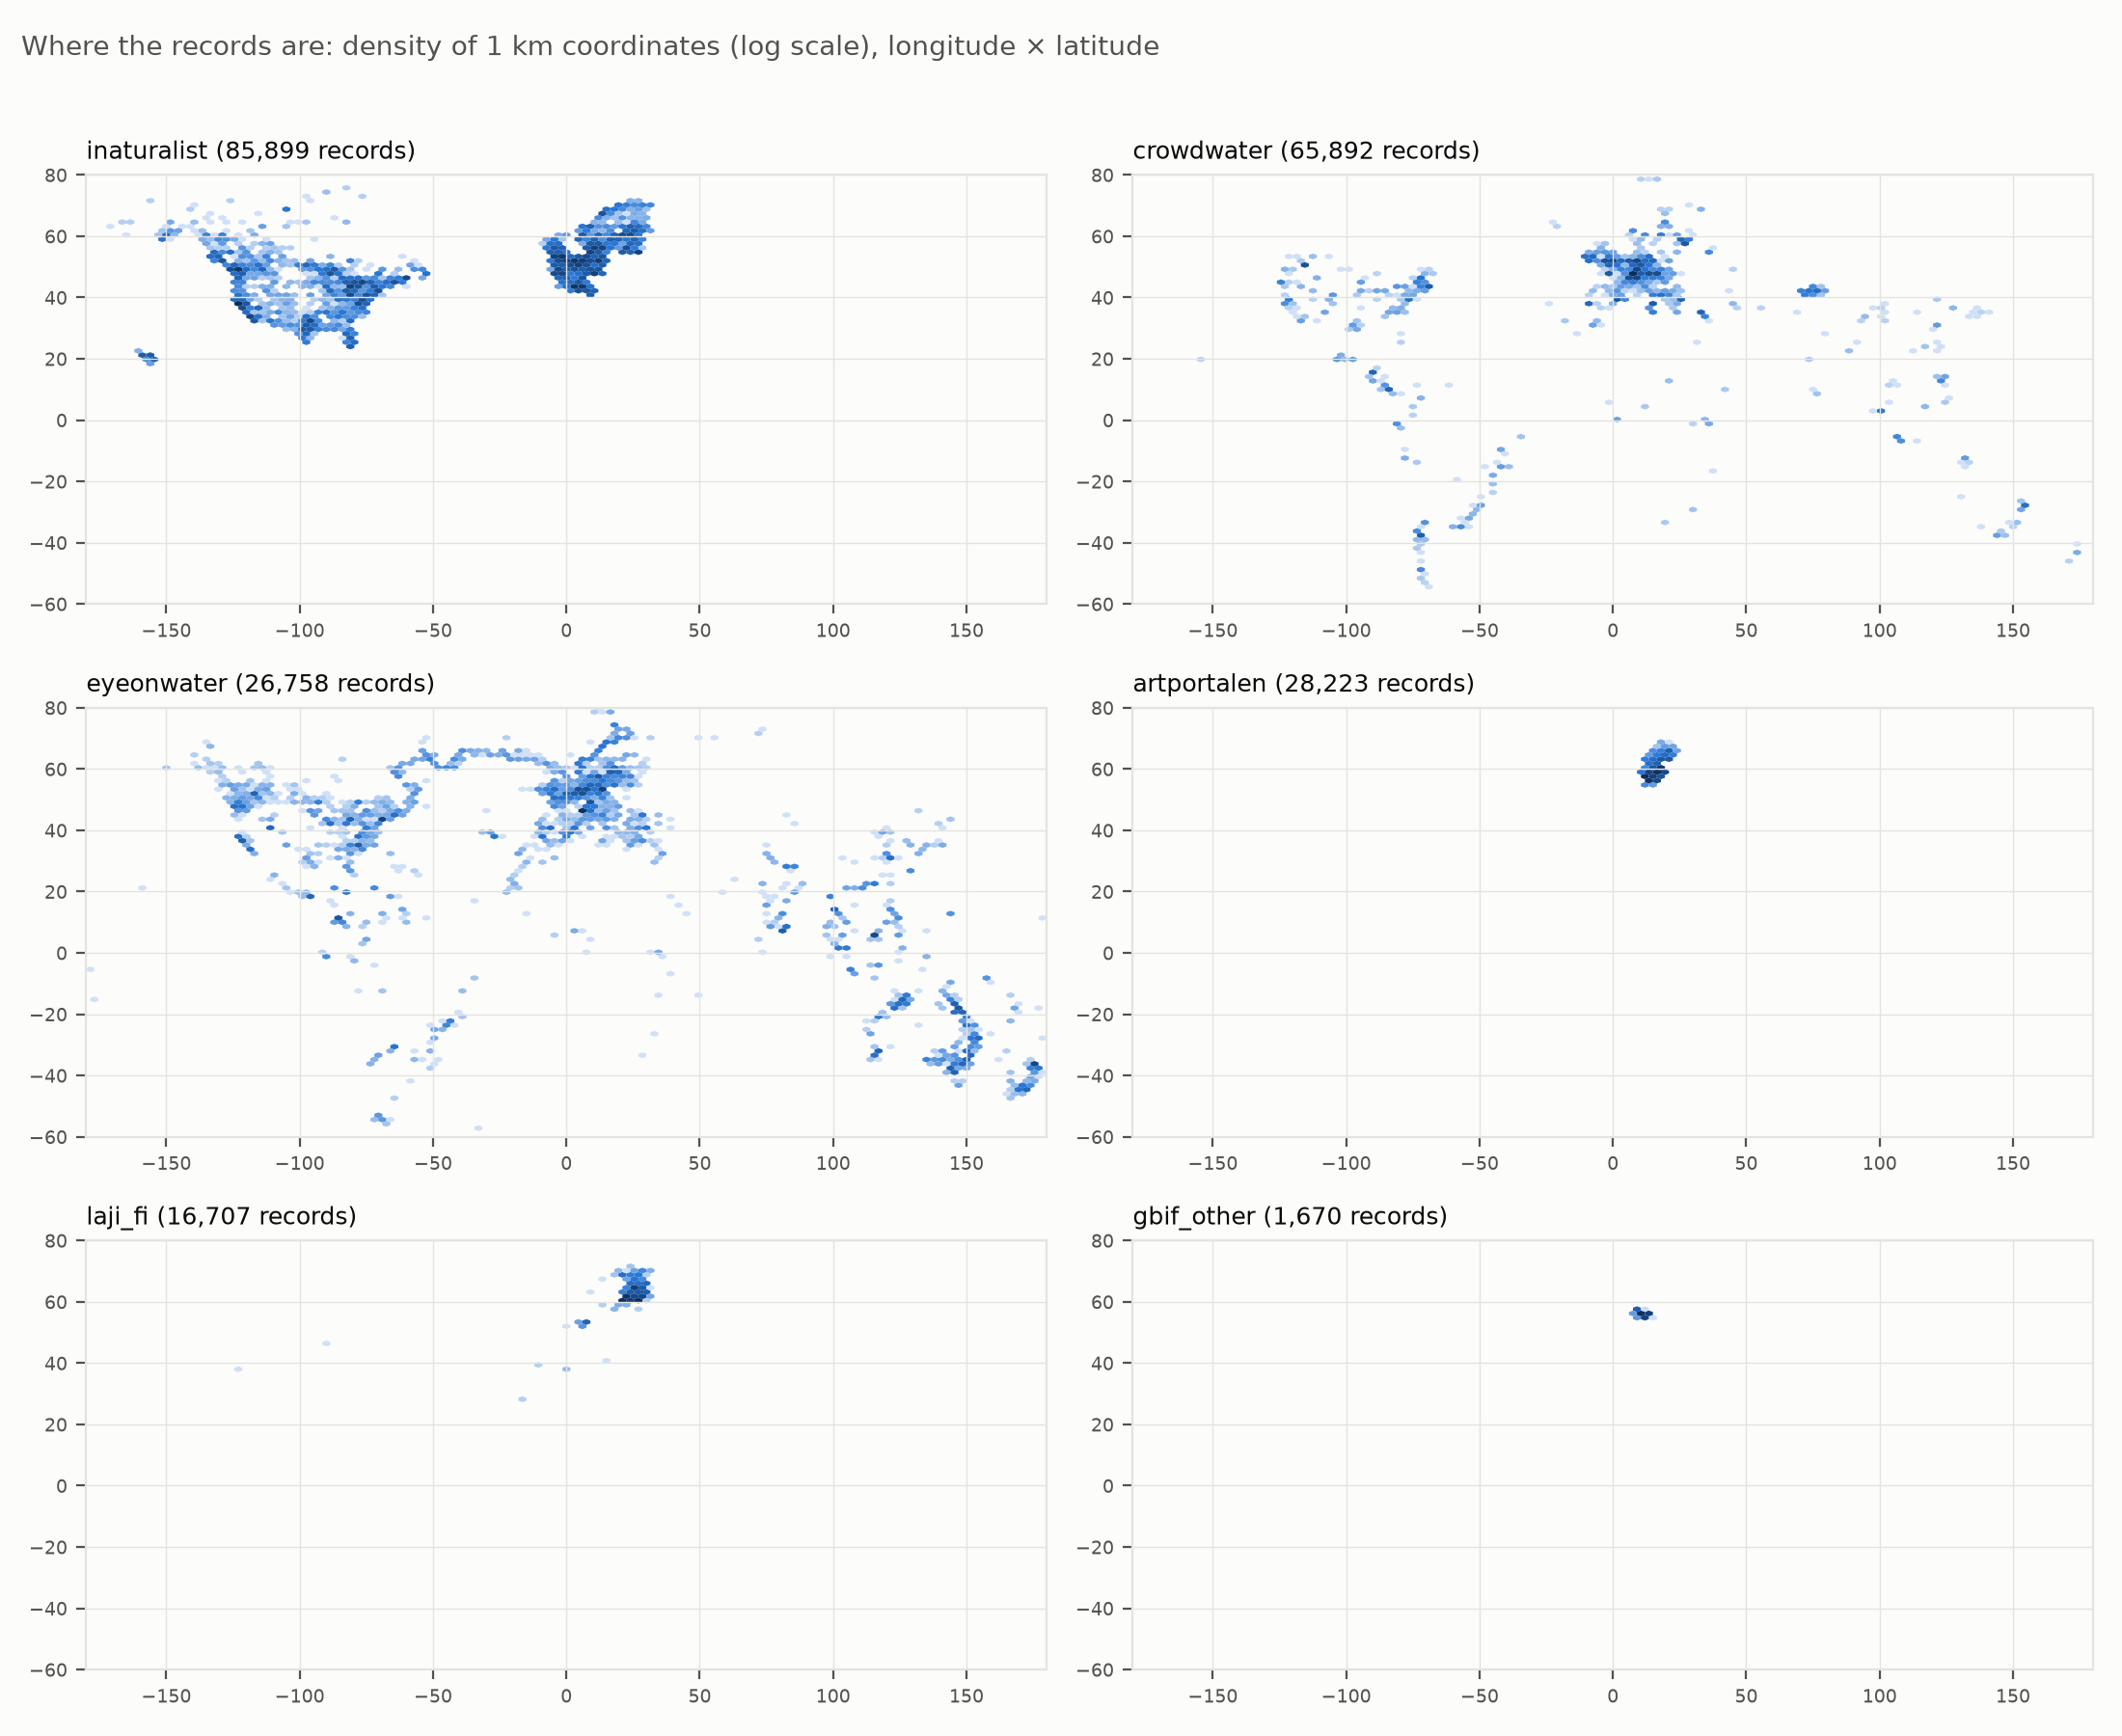
\includegraphics[width=0.72\textwidth]{spec11_map.png}
\caption{Where the records are: density of coordinates per platform (longitude $\times$ latitude).}
\label{fig:map}
\end{figure}

\begin{figure}[htbp]
\centering
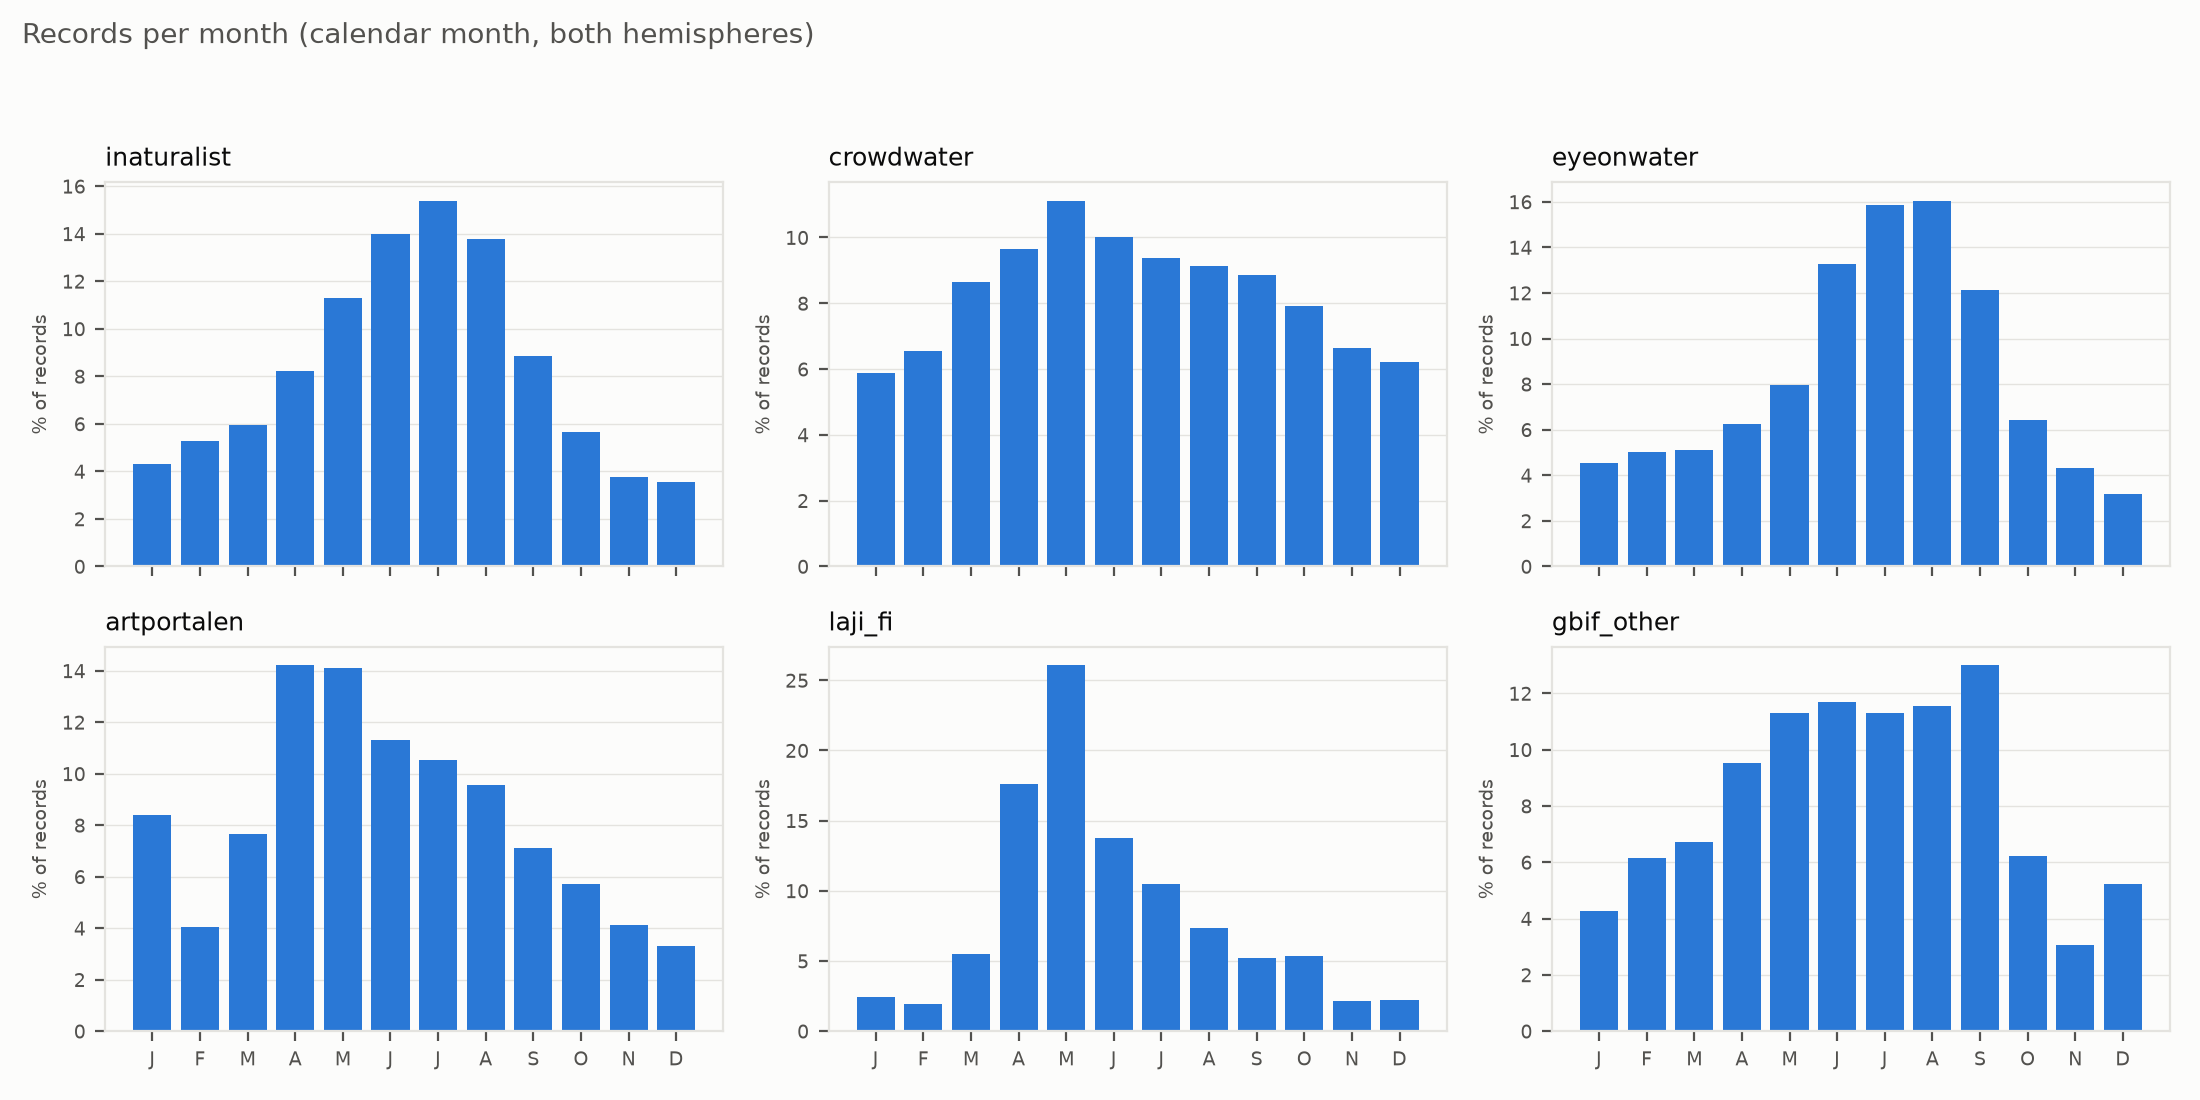
\includegraphics[width=\columnwidth]{spec11_months.png}
\caption{Share of records per calendar month, by platform.}
\label{fig:months}
\end{figure}

\section{Spec 14 --- Literature and limitations}

\textbf{Literature.} CrowdWater's virtual staff gauges~\cite{seibert2019crowdwater} and GBIF's national
portals~\cite{gbif} provide the structured data we build on; Kosmala et al.~\cite{kosmala2016quality} show that
citizen-science data can be reliable when quality is checked, which motivates our gold set and bias audit.
Our statistics follow Zipf~\cite{zipf1949human} and Heaps~\cite{heaps1978information}; agreement uses Cohen's
$\kappa$~\cite{cohen1960kappa}; the data card follows Datasheets for Datasets~\cite{gebru2021datasheets}. Beyond specs
2--9, the repository also contains a zero-shot LLM/VLM evaluation (Qwen2.5~\cite{qwen2024qwen25,bai2025qwen25vl};
68--69\% of checked outputs hallucinate, in the sense of~\cite{ji2023hallucination}) and a GLiNER
comparison~\cite{zaratiana2024gliner} that raises partial entity F1 from 0.44 to 0.52.


\textbf{Limitations.}
\begin{itemize}
  \item \emph{Gold design:} one student and one LLM per record (course guideline), not two students; student--student
        agreement comes only from the 20 calibration records.
  \item \emph{Split:} CrowdWater is 64/8/28 instead of 80/10/10, to keep each gauge in one split.
  \item \emph{Small numbers:} few positive gold labels (5 inconsistent image--text pairs, 4 turbid notes).
  \item \emph{Pipeline errors:} language identification fails on species names; translations are plausible but not
        always correct; the water filter is keyword-based (only 51\% of gold notes are about water).
  \item \emph{Coverage and privacy:} Latvian data is almost absent (non-commercial licences excluded); name masking
        misses a few names; photos are linked, not copied.
\end{itemize}
